\section{A two minute cycle}

We apply our proc-variance methods to a standard two-minute Bard rotation. We then compare this distribution to a fixed-proc rotation that uses the most likely proc counts. This quantifies how much extra damage variance procs contribute, and whether that variance matters in practice.

The rotation begins with The Wanderer's Minuet and accompanying burst window, analogous to any post-opener burst window. This window contains PP3 variability and Apex Arrow potency variability. The next song is Mage's Ballad, containing variable HS usages and variable Apex Arrow potency. Army's Paeon is the final song in this sequence and was found to have no song-specific variability for a 3-6-9 song sequence.

A few additional notes about the rotation:

\begin{itemize}
  \item The two minute window does not include snap-shot effects.
  \item All Heartbreak Shot procs granted during Mage's Ballad are used during Mage's Ballad to simplify buff accounting. This rotation may not perfectly count Heartbreak Shot usages.
  \item The damage-over-time ticks from Army's Paeon include the few ticks snap-shotted from the prior two minute window and the portion ticks from Army's Paeon in the current two minute window.
  \item When damage variability due to proc effects are present, the most likely number of usages are damage value is shown in the ``Fixed usage" column.
  \item Counts for values which are randomly distributed according to $P_X(n)$ are expressed as $\sim X(n)$. For example, Refulgent Arrow with a sub-sequence length of 14 would be expressed as $\sim RA(n=14)$.
  \item A counts involving a random variable transformation, like Burst Shot for a sub-sequence length for 14, is expressed as $14 - K_{ra} - 1; \: K_{ra} \sim RA(n=14)$.
\end{itemize}

The entire rotations also contains RA proc variability. Both rotation versions are tabulated in Table \ref{t:two-min-rotation}. 

\newpage
\onecolumn

% Increase page height by reducing top and bottom margins
\setlength{\topmargin}{-1.38in}     % More negative value = less top margin = more space
\setlength{\textheight}{9.5in}     % Larger value = more text area = less bottom margin
\setlength{\footskip}{0.3in}       % Smaller value = less space above footer

% Based off https://www.fflogs.com/reports/1nr8bqvTtBKPDwNW?fight=21
\begin{table}[]
\centering
\caption{Rotation for a 2 minute cycle.}
\label{t:two-min-rotation}
\begin{threeparttable}
\begin{tabular}{@{}lllll@{}}
\toprule
Action                    & D                      & No. usages                              & Fixed usage   & Buffs\tnote{a}          \\ \midrule
Refulgent Arrow           & 12,727                 & $\sim RA(n=2)$                          & 1             & \bufficons{wm} \\
Burst Shot                & 10,000                 & $2 - K_{ra}; \:  K_{ra} \sim RA(n=2)$   & 1             & \bufficons{wm} \\ \midrule
Refulgent Arrow           & 12,727                 & $\sim RA(n=1)$                          & 0             & \bufficons{wm,bv,rf} \\
Burst Shot                & 10,000                 & $1 - K_{ra}; \:  K_{ra} \sim RA(n=1)$   & 1             & \bufficons{wm,bv,rf} \\
Autos                     & 3,636                  & 1                                       &               & \bufficons{wm,bv,rf} \\
Heartbreak Shot           & 8,181                  & 1                                       &               & \bufficons{wm,bv,rf} \\ \midrule
Refulgent Arrow\tnote{b}  & 12,727                 & $3 + K_{ra}; \: K_{ra} \sim RA(n=3)$    & 3             & \bufficons{wm,bv,rf,rs} \\
Burst Shot                & 10,000                 & $3 - K_{ra} -1; \: K_{ra} \sim RA(n=3)$ & 1             & \bufficons{wm,bv,rf,rs} \\
Pitch Perfect (3)         & 16,363                 & $\sim PP3(n_{r}^b=8, n_r^{nb} = 7)$     & 3             & \bufficons{wm,bv,rf,rs} \\
Apex Arrow                & $D_{aa}(K_{sg})$\tnote{c} & 1                                   & D = 27,272    & \bufficons{wm,bv,rf,rs} \\
Autos                     & 3,636                  & 6                                       &               & \bufficons{wm,bv,rf,rs} \\
Heartbreak Shot           & 8,181                  & 3                                       &               & \bufficons{wm,bv,rf,rs} \\
Empyreal Arrow            & 11,818                 & 2                                       &               & \bufficons{wm,bv,rf,rs} \\
Blast Arrow               & 27,272                 & 1                                       &               & \bufficons{wm,bv,rf,rs} \\
Iron Jaws                 & 4,545                  & 1                                       &               & \bufficons{wm,bv,rf,rs} \\
Radiant Encore (3)        & 40,909                 & 1                                       &               & \bufficons{wm,bv,rf,rs} \\
Resonant Arrow            & 27,272                 & 1                                       &               & \bufficons{wm,bv,rf,rs} \\
Sidewinder                & 18,181                 & 1                                       &               & \bufficons{wm,bv,rf,rs} \\
Stormbite (tick)          & 1,136                  & 15                                      &               & \bufficons{wm,bv,rf,rs} \\
Caustic Bite (tick)       & 909                    & 15                                      &               & \bufficons{wm,bv,rf,rs} \\ \midrule
Refulgent Arrow           & 12,727                 & $\sim RA(n=1)$                          & 0             & \bufficons{wm,rs} \\
Burst Shot                & 10,000                 & $1 - K_{ra}; \:  K_{ra} \sim RA(n=1)$   & 1             & \bufficons{wm,rs} \\ \midrule
Pitch Perfect (3)         & 16,363                 & $\sim PP3(n_{r}^b=8, n_r^{nb} = 7)$     & 2             & \bufficons{wm} \\
Refulgent Arrow           & 12,727                 & $\sim RA(n=6)$                          & 2             & \bufficons{wm} \\
Burst Shot                & 10,000                 & $6 - K_{ra}; \: K_{ra} \sim RA(n=6)$    & 4             & \bufficons{wm} \\
Autos                     & 3,636                  & 5                                       &               & \bufficons{wm} \\
Heartbreak Shot           & 8,181                  & 1                                       &               & \bufficons{wm} \\
Empyreal Arrow            & 11,818                 & 1                                       &               & \bufficons{wm} \\ 
\midrule
\specialrule{0pt}{0pt}{0.8pt} % Zero-thickness rule with small vertical spacing
\midrule
Refulgent Arrow           & 12,727                 & $\sim RA(n=14)$                         & 4             & \bufficons{mb} \\
Burst Shot                & 10,000                 & $14 - K_{ra} - 1; \: K_{ra} \sim RA(n=14)$ & 9          & \bufficons{mb} \\
Apex Arrow                & $D_{aa}(K_{sg})$\tnote{c} & 1                                   & D = 27,272    & \bufficons{mb} \\
Heartbreak Shot           & 8,181                  & $3 + K_{hs}; \: K_{hs} \sim HS(n_r=14)$ & 6             & \bufficons{mb} \\
Autos                     & 3,636                  & 13                                      &               & \bufficons{mb} \\
Empyreal Arrow            & 11,818                 & 2                                       &               & \bufficons{mb} \\
Iron Jaws                 & 4,545                  & 1                                       &               & \bufficons{mb} \\
Sidewinder                & 18,181                 & 1                                       &               & \bufficons{mb} \\
Blast Arrow               & 27,272                 & 1                                       &               & \bufficons{mb} \\
Stormbite (tick)          & 1,136                  & 10                                      &               & \bufficons{mb} \\
Caustic Bite (tick)       & 909                    & 10                                      &               & \bufficons{mb} \\ 
\midrule
\specialrule{0pt}{0pt}{0.8pt} % Zero-thickness rule with small vertical spacing
\midrule
Refulgent Arrow           & 12,727                 & $\sim RA(n=17)$                         & 5             & \bufficons{ap} \\
Burst Shot                & 10,000                 & $17 - K_{ra} - 1; \: K_{ra} \sim RA(n=17)$ & 11         & \bufficons{ap} \\
Iron Jaws                 & 4,545                  & 1                                       &               & \bufficons{ap} \\
Autos                     & 3,636                  & 14                                      &               & \bufficons{ap} \\
Empyreal Arrow            & 11,818                 & 3                                       &               & \bufficons{ap} \\
Heartbreak Shot           & 8,181                  & 3                                       &               & \bufficons{ap} \\
Stormbite (tick)          & 1,136                  & 15                                      &               & \bufficons{ap} \\
Caustic Bite (tick)       & 909                    & 15                                      &               & \bufficons{ap} \\ \bottomrule
\end{tabular}
\vspace{3pt}

  \begin{tablenotes}\footnotesize
    \item[a] Buff legend: 
\includegraphics[height=1.1em]{img/icons/wm.png} = The Wanderer's Minuet;
            
\includegraphics[height=1.1em]{img/icons/bv.png} = Battle Voice;
            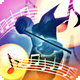
\includegraphics[height=1.1em]{img/icons/rf.png} = Radiant Finale;
            
\includegraphics[height=1.1em]{img/icons/rs.png} = Raging Strikes;
            
\includegraphics[height=1.1em]{img/icons/mb.png} = Mage's Ballad;
            
\includegraphics[height=1.1em]{img/icons/ap.png} = Army's Paeon.
    \item[b] Includes Refulgent Arrow under the effect of Barrage.
    \item[c] where $K_{sg} \sim SG(n_r=20)$.
  \end{tablenotes}
\end{threeparttable}
\end{table}

\newpage
\twocolumn
% Reset margins to default values
\setlength{\topmargin}{-0.55in}    % IEEEtran default
\setlength{\textheight}{9in}       % IEEEtran default
\setlength{\footskip}{0.5in}       % IEEEtran default (approximate)

Using the previously-developed methods, DPS distributions are computed for fixed and mixed rotations, Figure \ref{fig:two-min}. A time of $t=120$ seconds is assumed. 

\begin{figure}[H]
  \centering
  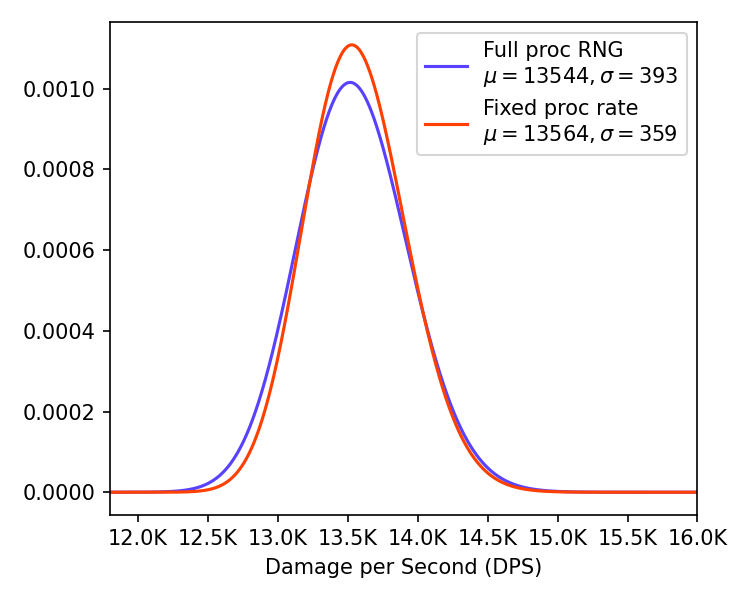
\includegraphics[scale=0.65]{img/full-rotation.png}
  \caption{DPS distribution for a 2-minute song sequence for a rotation fully accounting for procs, (blue) and a rotation assuming the most likely values (orange).}
  \label{fig:two-min}
\end{figure}

While procs can greatly influence the damage variability of particular actions, their effect on the damage variability for the whole rotation is quite small. The standard deviation only increases by 9.5\%, from 359 DPS to 393 DPS. Note that this is DPS for a two minute cycle. For realistic encounter durations, 6 - 18 minutes, the damage variability will be even lower. Interestingly, the damage variability manifests asymmetrically too, as the additional damage variability can largely be explained by an increase in probability for lower DPS values. In fact, accounting for procs has a miniscule effect on the likelihood of runs above the 50th percentile. Intuitively this makes sense as there is an 80\% chance for Repertoire to be granted, so any damage variability due to procs will result in lower DPS realizations. Additionally, the number of Refulgent Arrow / Burst Shot usages will be large and have relatively small variability, so using the most likely number of usages will often be sufficient for most use cases. From both a speed kill and parsing perspective, this means that whether procs are accounted for or not has no bearing enabling higher DPS runs. Accounting for procs, however, can more accurately account the likelihood of lower DPS runs.

Based on Figure \ref{fig:two-min}, Bard's action procs primarily serve as a gameplay mechanic that creates a more engaging rotation through decision-making opportunities. Correctly managing procs might even have a larger impact on the damage distributions than the number of procs granted. The minimal impact of proc variability on overall damage distributions leads to several practical implications for theorycrafting tools.

Most assumptions made here are based on perfect and idealized proc management, yet real-world factors will often violate these assumptions. Encounters, particularly Ultimate-level fights, can have unavoidable downtime that fundamentally alter proc distributions. Player execution factors (including buff misalignment, overcapped procs, rotational drift, and deaths) may also lead to significant deviations in ideal proc management. 

Prospective modeling tools like rotation planners may have an easier time reconciling with factors like downtime and can also assume perfect play. However, retrospective damage variability tools would have to account for the player execution aspect.\footnote{Disclaimer: I develop and maintain \href{https://howbadwasmycritinxiv.com}{https://howbadwasmycritinxiv.com}.} While it is theoretically possible to detect and account for these real-world factors, their implementation would be incredibly complex since it requires inferring and accounting for proc-based decision making from players. For most practical use cases, simply assuming the most probable proc counts provides sufficient accuracy for damage variability calculations while maintaining simplicity.